\chapter{Implementação e Validação} %não sei como chamar este capitulo
\label{chap:cap4}

Este capítulo apresenta uma ferramenta para a verificação de programas ROBO e um estudo de caso usado na validação da abordagem. A Seção \ref{sec:tool} apresentada a ferramenta que integra a abordagem de tradução, apresentada no Capítulo \ref{chap:cap3}, com o verificador de modelos FDR e retorna para o usuário o resultado da verificação através de sua interface gráfica. A Seção~\ref{sec:caso} apresenta um estudo de caso usado na validação da abordagem. O estudo de caso usa a ferramenta proposta para verificar um programa ROBO completo contendo variáveis e procedimentos.

\section{Ferramenta}
\label{sec:tool}

Esta seção descreve uma ferramenta desenvolvida na linguagem de programação Java\footnote[8]{https://java.com/download} com a finalidade de verificar automaticamente programas ROBO. Internamente, a ferramenta está estruturada conforme o Diagrama de Classes disposto na Figura~\ref{fig:diagrama}. A interface (\texttt{Checker}) possui três métodos: \texttt{translateRobo2CSP}, que recebe como entrada uma \textit{string} do programa escrito na linguagem ROBO e gera uma \textit{string} como saída; \texttt{translateMap2CSP} que recebe uma \textit{string} com a representação textual de um mapa do ambiente RoboMind e produz uma \textit{string}; e \texttt{verifyAssertion} que recebe como entrada o programa e o mapa na notação CSP e gera o objeto \texttt{Assertion}. A Classe \texttt{RobotChecker} implementa a Interface \texttt{Checker}. Essa classe possui alguns atributos que são responsáveis por armazenar informações importantes da tradução e da verificação. O atributo \texttt{programCSP} é utilizado para armazenar uma \textit{String} com a especificação formal CSP que representa o programa ROBO obtido como retorno do método \texttt{translateRobo2CSP}. A implementação deste método utiliza os serviços providos pelo \textit{framework} \texttt{Spoofax}. O atributo \texttt{mapCSP} armazena o texto que representa o CSP do mapa obtido como retorno do método \texttt{translateMap2CSP}. O método \texttt{verifyAssertion} chama métodos da API de FDR (representada pela classe \texttt{FDR}) passando como entrada as representações CSP para o programa e para o mapa gerado. O atributo \texttt{assertion} (instância da Classe \texttt{Assertion}) armazena em  \texttt{result} (se passou ou falhou) e \texttt{traces} (contraexemplo) o resultado da verificação automática. Para tornar transparente a tradução com Spoofax e a verificação com FDR para o usuário, desenvolvemos uma camada de apresentação que é representada pela Classe \texttt{GUI}. Destacamos alguns elementos desta classe. O atributo \texttt{btnProgram} representa um botão com a finalidade de buscar o programa ROBO fornecido pelo usuário. O atributo \texttt{btnMap} representa um botão para o usuário fornecer os mapas do RoboMind como entrada. O atributo \texttt{btnVerify} tem o intuito de iniciar o processo de tradução e posteriormente a verificação por meio da chamada do método \texttt{translator} da Classe \texttt{Controller} que recebe como entrada o programa e mapas do usuário e retorna o objeto \texttt{Assertion}. Os atributos \texttt{txtResult} e \texttt{txtTraces} são utilizados para exibir na tela da ferramenta o resultado da verificação e os \textit{traces} (contraexemplos) gerados pela verificação, respectivamente.

% Listamos as principais funcionalidades do protótipo implementado:

% \begin{itemize}
%     \item Tradução de ROBO para CSP: recebe um programa ROBO como entrada e através da API do Spoofax é realizada a tradução usando o compilador desenvolvido por esta pesquisa; e como saída é gerado a especificação do programa em notação CSP.
%     \item Tradução de mapa: recebe um mapa do ambiente RoboMind como entrada e realiza a tradução automática; e como saída é gerado a especificação formal em CSP do mapa.
%     \item Verificação das propriedades no FDR: recebe como entrada o mapa e o programa escritos em CSP, resultado da tradução automatizada; e como saída gera os resultados das verificações e os \textit{traces} resultantes, se houver.
% \end{itemize}

\begin{figure}[!h]
\centering
\caption{Diagrama de Classes do protótipo}
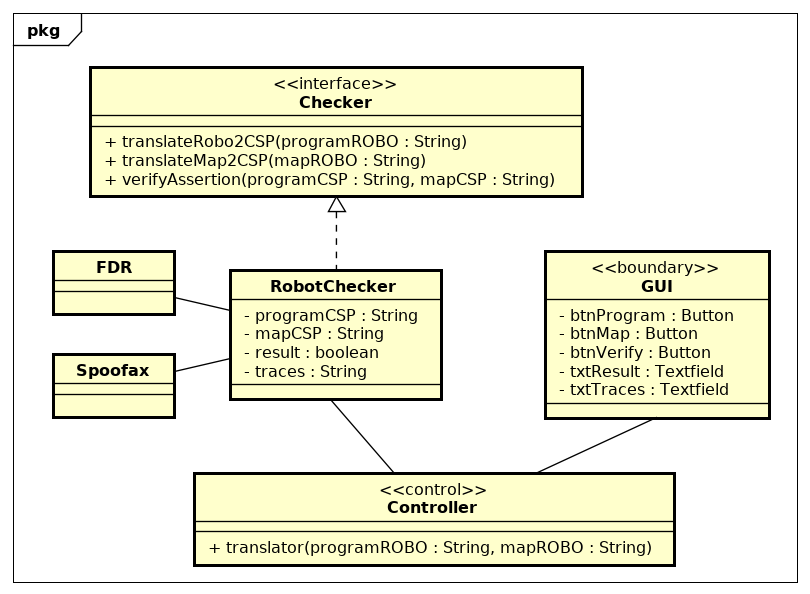
\includegraphics[height=8cm]{figuras/class_diagram.png}
\fonte{O autor}
\label{fig:diagrama}
\end{figure}

A Figura~\ref{fig:guiprot} mostra a Interface Gráfica (\textit{Graphical User Interface} - GUI) da ferramenta que implementa o diagrama mostrado anteriormente. A interface conta com três botões: ``Mapa'' onde o usuário escolhe um ou mais mapas do RoboMind, onde são listados abaixo; ``Programa'' onde o usuário seleciona o arquivo do programa ROBO, o nome do arquivo é posto abaixo dos botões; e no meio da tela está o botão ``Verificar`` que executa a tradução e em seguida a verificação. No lado direito da figura são listados os \textit{traces} (contraexemplos) gerados pela verificação. Na parte inferior da figura tem um \textit{console} para que o usuário tenha um \textit{feedback} do resultado da verificação automática.

\begin{figure}[!h]
\centering
\caption{Interface gráfica da ferramenta}
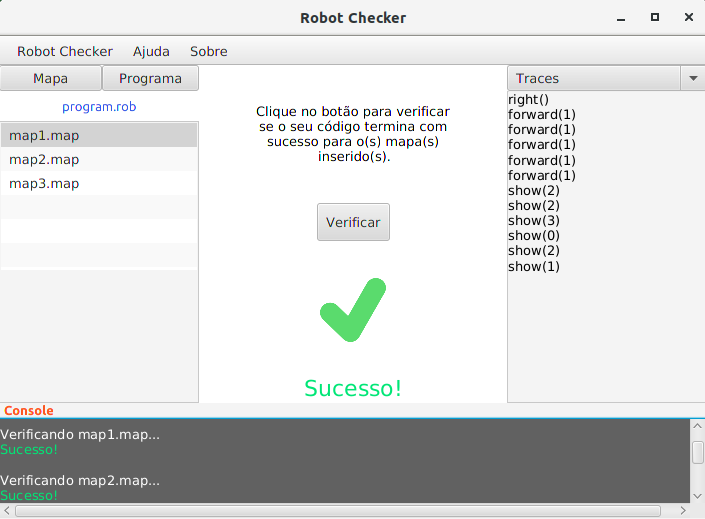
\includegraphics[height=8cm]{figuras/prototipo2.png}
\fonte{O autor}
\label{fig:guiprot}
\end{figure}

\section{Estudo de caso}
\label{sec:caso}

No Capítulo \ref{chap:cap3} foi apresentado parcialmente o exemplo (Contando Caixas), que é apresentado na íntegra nesta seção e  utilizado como estudo de caso para validar o processo de tradução e verificação automática.

O problema consiste em três mapas de 6 colunas e 3 linhas que possuem caixas distribuídas aleatoriamente na primeira e última linhas. Em todos os mapas, o robô inicia na primeira coluna da segunda linha e tem o objetivo de andar até a última coluna e parar. Após parar o robô, o programa mostra seis valores inteiros através do comando \texttt{show}. Os dois primeiros valores representam a quantidade de caixas encontradas na primeira e última linhas, respectivamente. O terceiro valor mostrado indica quais das linhas possui mais caixas: o valor 1 indica que a primeira linha possui mais caixas, o valor 2 que a última linha tem mais caixas, e o valor 3 que as linhas possuem a mesma quantidade de caixas. O quarto valor exibido é a diferença de caixas entre as duas linhas. O quinto valor indica em qual linha apareceu a primeira caixa: 1 se apareceu na primeira linha, 2 se apareceu na última linha; e 3 se apareceu em ambas as linhas. O sexto e último valor indica em qual linha apareceu a última caixa: 1 se apareceu na primeira linha, 2 se apareceu na última linha; e 3 se apareceu em ambas as linhas. Neste estudo de caso o programa ROBO foi verificado considerando os mapas apresentados na Figura \ref{fig:problem}. Nesta figura, no lado direito dos mapas mostra os valores esperados como saída pelo programa.

\begin{figure}[h]
\centering
\caption{Mapas e saídas esperadas do problema ``Contando Caixas"}
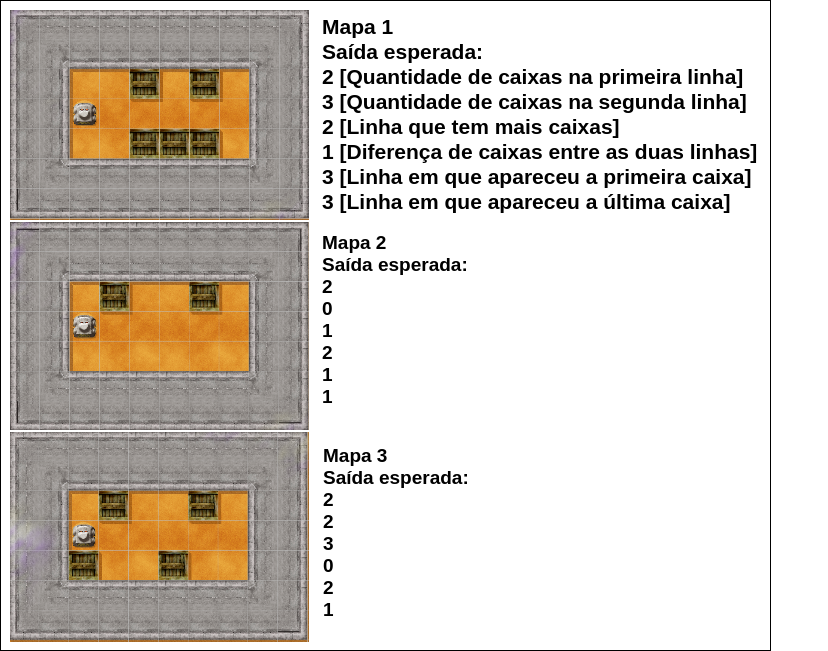
\includegraphics[height=10cm]{figuras/map_caso.png}
\fonte{\cite{furb}}
\label{fig:problem}
\end{figure}

Como solução candidata para o problema de contar caixas desenvolvemos o programa ROBO apresentado no Código~\ref{fig:solution}. Nas linhas 1 a 12 do código, estão declaradas as variáveis. As variáveis \texttt{countFirstLine} e \texttt{countLastLine} armazenam a quantidade de caixas encontradas pelo robô na primeira e última linhas, nesta ordem. As variáveis \texttt{findFirstBoxLeft} e\texttt{findFirstBoxRight} apontam quando a primeira caixa é encontrada na primeira e última linhas, respectivamente. As variáveis \texttt{firstBoxLeft} e \texttt{firstBoxRight} são utilizadas para armazenar a linha que aparece a primeira caixa. Já as variáveis \texttt{lastBoxLeft} e \texttt{lastBoxRight} armazenam a linha (primeira ou última) que aparece a última caixa. A quantidade de vezes que a instrução \texttt{forward} é executada é armazenada na variável \texttt{countForward}. Foram implementados alguns procedimentos para cada valor. O procedimento \texttt{countBoxes} (linhas 14 a 38) conta a quantidade de caixas à direita ou à esquerda do robô dependendo do valor do parâmetro \texttt{side}: valor 1 conta caixas a esquerda (primeira linha) e qualquer valor diferente de 1 conta caixas a direita (última linha). Para \texttt{side} igual a 1, esse procedimento incrementa em 1 a variável \texttt{countFirstLine} se à esquerda do robô tem obstáculo, isto é, se possui uma caixa. Em seguida, verifica se a variável \texttt{findFirstBoxLeft} é igual a 0, o que significa que ainda não encontrou a primeira caixa, e atualiza o valor de \texttt{firstBoxLeft} para a quantidade de comandos \texttt{forward} executados (\texttt{countForward}), assim, atualizando \texttt{findFirstBoxLeft} para o valor 1, indicando que a caixa da primeira linha foi encontrada. Essa explicação é análoga para \texttt{side} diferente de 1, o que significa que a verificação ocorre na última linha (à direita do robô). O procedimento \texttt{showsMoreBoxes} (linha 40 a 51) exibe no \textit{console} do RoboMind a linha com mais caixas e a diferença de caixas entre a primeira e última linha. O procedimento \texttt{getBoxFirstLine} (linhas 53 a 61) exibe qual das linhas há uma ocorrência da primeira caixa. Já o procedimento \texttt{getboxLastLine} (linhas 63 a 71) exibe o valor correspondente à linha no qual a última caixa aparece. As instruções que iniciam o programa estão dispostas nas linhas 73 a 88. O primeiro comando é \texttt{right}, que altera a orientação do robô para a direção leste. O comando seguinte é o laço \texttt{repeatWhile} que executa os comandos em seu corpo enquanto não existe um obstáculo à frente do robô. No escopo desse laço, há duas chamadas para o procedimento \texttt{countBoxes}, os valores 1 e 2 são passados no parâmetro para verificar à esquerda e à direita do robô, respectivamente. A próxima instrução é um \texttt{forward} para movimentar o robô uma célula à frente e em seguida incrementar o valor de \texttt{countForward} em 1. Ao sair do laço, o programa executa novamente o procedimento \texttt{countBoxes} para verificar na célula onde o robô parou, se há ocorrência de caixas na primeira e última linhas. As próximas instruções são para exibir as saídas do programa no \textit{console} do ambiente RoboMind: \texttt{show(countFirstLine)} e \texttt{show(countLastLine)} exibem o primeiro e segundo valor; a chamada do procedimento \texttt{showsMoreBoxes} exibe o terceiro e quarto valor; a chamada do procedimento \texttt{getBoxFirstLine} exibe o quinto valor; e \texttt{getBoxLastLine} exibe o sexto valor.

\lstinputlisting[caption=Solução proposta em ROBO para o problema Contando Caixas, label=fig:solution,numbersep=8pt]{codes/solution_completa.rob}
\fonte{O autor}


%Para validar a efetividade do compilador integrado ao FDR, foi necessário verificar as saídas geradas pelo protótipo e executar os \textit{traces} no ambiente RoboMind, obtidos através do resultado da verificação da propriedade: \texttt{assert PROGRAM :[deadlock free [F]]}.

Para validarmos a ferramenta implementada, utilizamos como entrada os três mapas apresentados na Figura~\ref{fig:problem} e o programa mostrado no Código~\ref{fig:solution}. Expomos em tabelas as entradas e saídas para cada dos métodos da classe \texttt{RobotChecker}. Na Tabela~\ref{table:map1}, \texttt{program.robo} é a entrada para o método \texttt{translateRobo2CSP} e como saída é gerado a especificação formal em CSP (\texttt{program.csp}). No método \texttt{translateMap2CSP}, map1.map é o arquivo de entrada, e map1.csp é a saída gerada pela tradução do mapa na notação de CSP. No método \texttt{verifyAssertion}, a notação CSP do mapa e do programa são entradas para a verificação (\texttt{program.csp} e \texttt{map1.csp}). Além dessas entradas, também é incluído \texttt{test1\_program\_map1.csp}, responsável por incluir os arquivos CSP utilizados na verificação, este é gerado durante a execução do método. Na Figura~\ref{fig:test} é mostrado o conteúdo do arquivo \texttt{test1\_program\_map1.csp} que é dado como entrada para FDR realizar a verificação. Neste arquivo, as linhas 1 a 3 incluem as especificações do modelo, do mapa e do programa usando o comando \texttt{include} de FDR. Na linha 5 está disposto a propriedade a ser verificada por FDR (\texttt{assert PROGRAM :[deadlock free [F]]}) que corresponde a verificação se o programa está livre de \textit{deadlock}. As saídas do método \texttt{verifyAssertion} são o resultado da verificação da propriedade (\texttt{result1}) e os traces gerados (\texttt{traces1}). As explicações mencionadas são análogas para a Tabela~\ref{table:map2} e para a Tabela \ref{table:map3}.

\begin{figure}[h]
\centering
\caption{Exemplo de entrada para a verificação no FDR}
\lstinputlisting[nolol]{codes/test.csp}
\fonte{O autor}
\label{fig:test}
\end{figure}

\begin{table}[h]
\caption{Entradas e saídas para o mapa 1}
\resizebox{\textwidth}{!}{%
\begin{tabular}{*{14}{|c}|}
\hline
\multicolumn{3}{|c|}{\textbf{Map 1}} \\ \hline
\textbf{method} & \textbf{input} & \textbf{output} \\ \hline
translateRobo2CSP & program.robo & program.csp \\ \hline
translateMap2CSP & map1.map & map1.csp \\ \hline
verifyAssertion & program.csp, map1.csp, test1\_program\_map1.csp & result1, traces1 \\ \hline
\end{tabular}%
}
\label{table:map1}
\fonte{O autor}
\end{table}

\begin{table}[h]
\caption{Entradas e saídas para o mapa 2}
\resizebox{\textwidth}{!}{%
\begin{tabular}{*{14}{|c}|}
\hline
\multicolumn{3}{|c|}{\textbf{Map 2}} \\ \hline
\textbf{method} & \textbf{input} & \textbf{output} \\ \hline
translateRobo2CSP & program.robo & program.csp \\ \hline
translateMap2CSP & map2.map & map2.csp \\ \hline
verifyAssertion & program.csp, map2.csp, test2\_program\_map2.csp & result2, traces2 \\ \hline
\end{tabular}%
}
\label{table:map2}
\fonte{O autor}
\end{table}

\begin{table}[h]
\caption{Entradas e saídas para o mapa 3}
\resizebox{\textwidth}{!}{%
\begin{tabular}{*{14}{|c}|}
\hline
\multicolumn{3}{|c|}{\textbf{Map 3}} \\ \hline
\textbf{method} & \textbf{input} & \textbf{output} \\ \hline
translateRobo2CSP & program.robo & program.csp \\ \hline
translateMap2CSP & map3.map & map3.csp \\ \hline
verifyAssertion & program.csp, map3.csp, test3\_program\_map3.csp & result3, traces3 \\ \hline
\end{tabular}%
}
\fonte{O autor}
\label{table:map3}
\end{table}

Utilizando a ferramenta apresentada na Figura~\ref{fig:guiprot}, selecionamos os três mapas apresentados na Figura~\ref{fig:problem} e o programa apresentado no Código~\ref{fig:solution} como entrada. Executamos a verificação e obtivemos os resultados apresentados na Tabela~\ref{table:results}. Para os três mapas o resultado da propriedade \texttt{assert PROGRAM :[deadlock free [F]]} falhou, o que significa que para cada um dos mapas o programa ROBO possui \textit{deadlock}, portanto, o programa termina sua execução em todos os mapas. Os contraexemplos gerados (\textit{traces}) para os três mapas possuem os seis primeiros eventos iguais.  Inicialmente, possuem o evento \texttt{right}, pois a primeira instrução do programa é virar a direita. Em seguida, realizam um laço que avança a posição do robô enquanto não há uma parede na frente do robô. Como resultado, o trace apresenta cinco vezes o comando \texttt{forward}. Os eventos que diferem entre os mapas são os eventos (\texttt{show}). Analisando o valor dos eventos \texttt{show}, pode-se confirmar que os mapas apresentaram as mesmas saídas apresentadas na Figura~\ref{fig:problem}. As saídas produzidas pela verificação foram comparadas com as saídas apresentadas no \textit{console} do ambiente RoboMind após concluir a execução do mesmo programa. Com esta comparação pode-se confirmar que o resultado da simulação em RoboMind foi idêntico ao resultado mostrado na verificação. O que mostra que o o modelo, para o programa analisado, captura a mesma semântica da simulação de RoboMind.

\begin{table}[H]
\caption{Resultado da verificação usando a  ferramenta proposta}
\resizebox{\textwidth}{!}{%
\begin{tabular}{*{14}{|c}|}
\multicolumn{1}{c}{Map 1} & \multicolumn{1}{c}{Map 2} & \multicolumn{1}{c}{Map 3} \\
assert PROGRAM :{[}deadlock free {[}F{]}{]} & assert PROGRAM :{[}deadlock free {[}F{]}{]} & assert PROGRAM :{[}deadlock free {[}F{]}{]} \\
Result: Failed & Result: Failed & Result: Failed \\
Counterexample - Traces: & Counterexample - Traces: & Counterexample - Traces: \\
right() & right() & right() \\
forward(1) & forward(1) & forward(1) \\
forward(1) & forward(1) & forward(1) \\
forward(1) & forward(1) & forward(1) \\
forward(1) & forward(1) & forward(1) \\
forward(1) & forward(1) & forward(1) \\
show(2) & show(2) & show(2) \\
show(3) & show(0) & show(2) \\
show(2) & show(1) & show(3) \\
show(1) & show(2) & show(0) \\
show(3) & show(1) & show(2) \\
show(3) & show(1) & show(1)
\end{tabular}%
}
\fonte{O autor}
\label{table:results}
\end{table}

Tendo em vista os resultados no estudo de caso, podemos afirmar que a abordagem proposta por este trabalho, apesar das suas limitações, é capaz de verificar o comportamento de programas ROBO. 
%Além disso, vimos a possibilidade de integrar o compilador com o verificador de modelos por meio de uma ferramenta que realiza a verificação de modo transparente ao usuário. Sendo assim, um modo efetivo para auxiliar alunos e professores ao utilizar o ambiente RoboMind.


